\section{Talking to Machines}

After researching microworlds and developing my theoretical framework, I
felt ready to design my own microworld, which I named \emph{Talking to
Machines}. You can find it online at \url{http://draw.talkingtomachines.org}.

Concretely, this entailed designing an environment in which an
\textbf{idea-implementation-evaluation} loop could be carried out. For the
reasons discussed in the previous section, I decided to host this
environment within the web browser.

This decision brought with it some constraints: the interface would have
to be built from HTML and CSS, and interactivity would have to either be
supplied by client-side JavaScript, or a server-side evaluation
environment. But this decision also enabled the increased accessibility
discussed earlier.

I decided to focus this microworld on programming, as that is an
activity I have a lot of experience with. In a web environment, that
would entail using JavaScript as the programming language, as that is
available on the client-side, and removes the need to execute a
different language on the server and then send back the results.

However, I'm not a great fan of JavaScript when it comes to teaching
beginners to program (see \href{https://www.destroyallsoftware.com/talks/wat}{here}\footnote{https://www.destroyallsoftware.com/talks/wat} for why, from 1:18). Instead, I chose to use
a dialect of Lisp - Clojure (in its JavaScript-hosted form,
ClojureScript) - as Lisp has a history of being a language well-suited
for beginners (MIT has used it in an introductory \href{http://mitpress.mit.edu/sicp/course.html}{programming course}\footnote{http://mitpress.mit.edu/sicp/course.html} for years).

\subsection{From ClojureScript to JavaScript}

At the time of creating \emph{Talking to Machines}, there was no way to
dynamically evaluate ClojureScript in the browser, as the reader and
compiler for ClojureScript forms was in fact a Clojure program that
could only run on the Java Virtual Machine.

The following makes this rather complicated concept a little easier to
understand:

The ClojureScript syntax for printing ``Hello World!'' to the console
looks like this: 

\begin{verbatim}
(.log js/console 'Hello World!')
\end{verbatim}

If ClojureScript could be evaluated in the browser, you'd expect to be
able to do something like this, in \textbf{JavaScript}: 

\begin{verbatim}
ClojureScript.eval("(.log js/console 'Hello World!')") 
\end{verbatim}

and have ``Hello World!'' printed to the console.

Unfortunately, in standard ClojureScript, you can't do that yet.

Instead, a \textbf{Clojure} program, running on the JVM (i.e. not in the browser), has to \textbf{transpile} a ClojureScript file to a
JavaScript file. This means that 

\begin{verbatim}
(.log js/console "Hello World!")
\end{verbatim}

in the Clojurescript file, \texttt{foo.cljs}, is transpiled to

\begin{verbatim}
console.log("Hello World!")
\end{verbatim}

in the output Javascript file, \texttt{foo.js}, by a server-side process run during a compilation phase. 

It is this file, \texttt{foo.js}, that is later evaluated in the web browser.

\subsection{So what does this mess actually mean, practically?}

It means that if a user writes ClojureScript in the browser, we won't be
able to evaluate what they wrote without having a backend Clojure
process transpiling their code to JavaScript for us.

This isn't actually a massive issue, as we still don't evaluate
arbitrary code on the back-end, which would obviously be a Big Deal (we
only transpile it), but it would introduce some network lag
between the \textbf{implementation} and \textbf{evaluation} stages of
our microworld loop.

We know the tighter the microworld loop, the more engaging the experience, so lag was something I wanted to avoid if at all possible.

\subsubsection{Kanaka to the rescue}

Luckily for me, there was a \href{https://github.com/kanaka/clojurescript}{fork of ClojureScript}\footnote{https://github.com/kanaka/clojurescript} that did allow evaluation in the browser, written by Joel Martin
(``Kanaka'' on Github). At the time of writing it is still a fork, and
hasn't been merged with ClojureScript core, probably because it contains
``miscellaneous broken things that have not been tracked down yet''.

But it was definitely good enough to evaluate ClojureScript for a
microworld, and it probably took me less time to modify Martin's code to
provide my wished-for \texttt{ClojureScript.eval} JavaScript function
than it took me to explain why that was necessary.

\subsection{Why did I go to all this trouble?}

This might seem like a very convoluted mess to get into just to avoid
writing pure JavaScript, which, after all, is good enough for sites like
\href{http://codecademy.com}{Codecademy}\footnote{http://codecademy.com}. That's a fair point but I believe that the declarative
purity of ClojureScript forms makes up for the chaos going on behind the
scenes. As you will soon see.

\subsection{A better first impression of programming}

Most very-first-introductions to a programming language, or programming
in general, involve printing the text ``Hello World!'' to the screen.
Later exercises usually include things like printing the numbers ``1 2 3
4 5 6 7 8 9 10'', or adding up all integers less than 100.

Though these feats may have been impressive 30 years ago, today these things fail to blow
most people's socks off.

Producing plaintext is far from unimportant (most webservers do little
else), but in a world where technology means Oculus Rift and 4K Netflix,
it's not really sexy.

Is there something simple we can have beginners do, to explain functions
and variables and loops, that is more interesting than printing text to
the screen?

We could try the activity that captivates children (and artists) all
over the world: drawing things. With colours!

\begin{figure}[ht!]
\centering

\includegraphics[width=100mm]{img/concentric_circles.png}
\caption{The kind of thing that blows socks off.}
\label{overflow}
\end{figure}

\subsection{Declarative shapes}

The most basic form of computation is a single function call. It is the
simplest action that \emph{does} something (variable assignment does
something too, but indirectly, setting things up for later function
calls).

It makes sense that drawing a shape to a screen should be the result of
just one function call, instead of requiring a novice to construct a
class, call methods on that class, and then draw that class to the
screen after having acquired a graphics context.

The more declarative this function call, the easier it is for a novice
to deduce its meaning from what happens when its evaluated.

Consider: 

\begin{verbatim}
(circle
 (position "50%" "50%")
 (radius 100)
 (fill "red"))
\end{verbatim}

To a non-programmer (and perhaps even a programmer unused to
S-expressions), this line of text looks alien. It conforms to a very
different kind of grammar than what we're used to reading.

This is why, when I ask non-programmers what they think the \texttt{100} in
the line above represents, they often have no idea. The text as a whole
is just too strange for them to parse and guess that the proximity of
\texttt{radius} to \texttt{100}, and the brackets that enclose them, means that the
two tokens have something to do with each other.

If we were in a static environment, the only way to learn about what the
above text does would be to read about the syntax and grammar of Lisp, and the semantics of \emph{Talking to Machines}.
This is often how programming is approached: from a mathematical
perspective. The only way to find out if you had a correct understanding
of syntax, grammar and semantics would be to ask a teacher. The gap between
\textbf{implementation} and \textbf{evaluation} would be so large that
it would kill a lot of your motivation.

Fortunately, \emph{Talking to Machines} is a microworld. This means that
a student can \textbf{evaluate} the above text, right in the browser, to render:

\begin{figure}[ht!]
\centering

\includegraphics[width=20mm]{img/red_circle.png}
\caption{The meaning of the S-expression}
\label{overflow}
\end{figure}

Then, after processing this visual feedback, the student might have an idea about what the \texttt{(radius 100)} form does, and decide to implement her idea by changing that form to \texttt{(radius 200)}. 

\begin{verbatim}
(circle
 (position "50%" "50%")
 (radius 200)
 (fill "red"))
\end{verbatim}

\begin{figure}[ht!]
\centering

\includegraphics[width=60mm]{img/big_red_circle.png}
\caption{Doubling the radius to 200}
\label{overflow}
\end{figure}

As soon as this modified text is \textbf{evaluated}, a \emph{bigger} circle is drawn on the screen. Immediately, the student realises
that the number that was \texttt{100} but is now \texttt{200} somehow affects the
\emph{size} of the drawn circle.

Through their interactions, the student has \textbf{constructed} this
knowledge for themselves. According to our constructionist learning
theory, this knowledge should be far more effective than being
\emph{told} that the \texttt{(radius 100)} form controls the radius of
the drawn circle.

\subsection{Looping in \emph{Talking to Machines}}

Let's see how \emph{Talking to Machines} supports our microworld loop.

Once a student is somewhat familiar with how the microworld works, they
can come up with the following \textbf{ideas}: 

\begin{itemize}
\item I want to draw a red circle. 
\item Can I make it blue? 
\item Can I make it bigger?
\item Can I move it around? 
\item Can I draw more than one? 
\item Can I draw other shapes? 
\item Can I animate them?
\item etc.
\end{itemize}

Their \textbf{implementations} of these ideas take the form of composed
function calls. These function calls are immediately \textbf{evaluated},
and the student sees visually how their change of code affected the
change in what was drawn to the screen.

\begin{figure}[ht!]
\centering
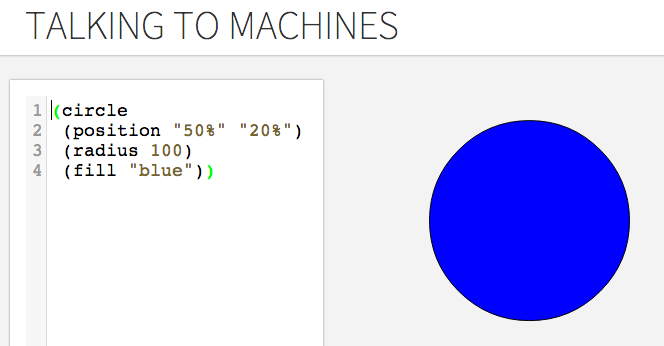
\includegraphics[width=115mm]{img/ttmachines_interface.png}
\caption{The Talking to Machines microworld interface}
\label{overflow}
\end{figure}

For example, the first idea above, of drawing a red circle, looks like
this: 

\begin{verbatim}
(circle (position 50% 50%) (radius 100) (fill "red"))
\end{verbatim}

Making it blue looks like this:

\begin{verbatim}
(circle (position 50% 50%) (radius 100) (fill "blue"))
\end{verbatim}

Making it bigger:

\begin{verbatim}
(circle (position 50% 50%) (radius 200) (fill "blue"))
\end{verbatim}

Moving it around: 

\begin{verbatim}
(circle (position 10% 50%) (radius 200) (fill "blue"))
\end{verbatim}

As we can see, the student iterates the following loop \emph{extremely fast}: 

\begin{enumerate}
\item Hmm, what does this do? (idea) 
\item I'll tweak it! (implementation) 
\item Ah, that's what that does! (evaluation) 
\item Hmm, but what about \emph{this}? (GOTO 1) 
\end{enumerate}

This keeps engagement high.

The student learns something new on every iteration, which feels rewarding,
which pushes them to iterate again.

\subsection{Limitations of this microworld}

\emph{Talking to Machines} was a success on a \emph{structural} level,
but a failure on a \emph{practical} level, at least given the time
constraints of this thesis.

It successfully enabled the learning iterations of a microworld, but it
required students to have too much prior knowledge for me to be able to
conduct workshops with many students at once.

It is possible for students of \emph{Talking to Machines} to learn Lisp syntax through trial and error, by
chopping and changing parentheses until the code evaluates. But this is
not the most efficient way to learn syntax, so engagement suffers as a
result.

Instead, students could be guided through their first attempts to
produce syntactically correct code, for example, being told: 

\begin{quote}
A Lisp function call has the form \texttt{(f x)} where \texttt{f} is a function and \texttt{x} is the argument. Try calling the \texttt{circle} function with the argument \texttt{50}!
\end{quote}

This kind of guidance takes time to do well, either by employing many
human assistants with the skill to teach students about syntax, or by
programming a tutorial in which the computer itself guides the student.

I didn't have this kind of time. Ideally, I wanted to explore the
knowledge-constructing effects of microworlds on students, without
having to teach them a new syntax beforehand.

This is what led me to create another microworld, which will be the focus of the next section.
